\subsection{Comparison Analysis}
\label{subsection: comparison}
Given the preliminary geometry of the aircraft, the mass properties of the aircraft's sections were calculated and tabulated in Table \ref{tab:mass_props}. Equations used and analyzed came from Raymer \cite{raymer} and Roskam Part V \cite{roskam_5}, class II analysis for traditional construction of aircraft. To account for the use of composites in the wing, horizontal and vertical stabilizers, a correction factor of 0.8* was applied, the weight savings quoted by Boeing Commercial Aircraft for composite aircraft structure over aluminum structure, was applied to estimations for the aircraft's lifting surfaces \cite{bcacomposite}.  Finally, an actual weight was chosen by either an average or closest value to the estimated weight from the seed aircraft (777-200) given the seed inputs.

\begin{table}[!h]
\centering
\caption{Independent Mass Estimations of SAM Mk I}
\begin{tabular}{|c||c|c|c|c| }
\toprule
\multicolumn{1}{|c||}{\textbf{Description}} & \multicolumn{1}{c|}{\textbf{Raymer Weight}} &  
 \textbf{Roskam Weight} & \textbf{Design Weight} & \textbf{Equation Used} \\ \hline \hline 
Wing & 32,000* & 31,600* & 31,600* & Roskam 5.6  \cite{roskam_5} \\ \hline
Fuselage & 61,600 & 41,900 & 41,900 & Roskam 5.27  \cite{roskam_5} \\ \hline
Horizontal Stabilizer & 6,000* & 9,800* & 9,900* & Roskam 5.19 \cite{roskam_5} \\ \hline
Vertical Stabilizer & 2,500* & 3,900* & 3,900* & Roskam 5.20 \cite{roskam_5} \\ \hline
Main Landing Gear & 4,100 & 11,900 & 11,900 & Roskam 5.42  \cite{roskam_5} \\ \hline
Nose Landing Gear & 450 &2,400 & 2,400 & Roskam 5.42  \cite{roskam_5} \\ \hline
Fixed Equipment & 55,000 & 65,000 & 60,000 & Roskam V Pgs. 97-111 \cite{roskam_5}  \\
& & & & \& Raymer Pgs. 575-576 \cite{raymer} \\ \hline
Engine Weight (per) &  \multicolumn{4}{|c|}{19,316}   \\ \hline
Baggage Weight & \multicolumn{4}{|c|}{12,300 (30 lbs/occupant) }  \\ \hline
Payload Weight & \multicolumn{4}{|c|}{82,000 (200 lbs/occupant) }  \\ \hline
Total Fuel Weight & \multicolumn{4}{|c|}{146,860 (6.71 lbs/gal) }  \\ \hline \hline
\textbf{Empty Weight} & 160,326 & 217,371 & \textbf{216,200} & -\\ \hline
\textbf{MTOW} & 364,626 & 421,671 & \textbf{443,800}  & - \\ \hline
\textbf{MZFW} & 242,326 & 299,371 & \textbf{310,500}  & - \\ \hline
\textbf{MLW} & 168,165 & 219,197 & \textbf{388,400} & - \\
\bottomrule
\end{tabular}
\label{tab:mass_props}
\end{table}
\FloatBarrier

It was found that Roskam, specifically the General Dynamics and Torenbeek methods, estimated the weight of the structure and landing gear with a smaller percentage of error when calculating MTOW for the 777-200 and other seed aircraft than the Raymer equations. Because of the higher fidelity of the structure and landing gear weight given by Roskam, Roskam class II was utilized for those sections. Fixed equipment, which consists of systems, avionics, fuel systems, and other miscellaneous necessities of the aircraft, was estimated using the average between Raymer and Roskam build-ups. The engine, the GE90-115B, weight is a direct value from the manufacturer \cite{roskam_5} \cite{raymer}.

\clearpage
\subsection{Center of Gravity}
The center of gravity (CG) of the aircraft was also estimated using the class II estimation methods found in Roskam Part V and Raymer.\cite{roskam_5}\cite{raymer} In Table \ref{tab:cg}, the CG locations of each major component is tabulated. Note that the locations in the table are referenced from the aircraft's coordinate, which is located 23.3 feet forward and 36.5 feet below the nosecone of the aircraft seen in Fig. \ref{fig:master_coord_def}.

\begin{table}[!h]
\centering
\caption{CG Locations of Primary Structures and Systems}
\begin{tabular}{|l||l|l|l|}
\hline 
                         & \textbf{X Location (ft)} & \textbf{Z Location (ft)} & \textbf{Equation Used}                                                     \\ \hline\hline
\textbf{Wing}            & -135.2                   & 33.8                    & Roskam Table 8.1                                                            \\ \hline
\textbf{Fuselage}        & -128.3                   & 38.0                    & Roskam Table 8.1                                                            \\ \hline
\textbf{H-Stab}          & -235.4                   & 39.9                    & Roskam Table 8.1                                                            \\ \hline
\textbf{V-Stab}          & -228.7                   & 56.2                    & Roskam Table 8.1                                                            \\ \hline
\textbf{Main Gear (ext)} & -23.3                    & 26.3                    & Roskam Table 8.1                                                            \\ \hline
\textbf{Nose Gear (ext)} & -23.3                    & 26.3                    & Roskam Table 8.1                                                            \\ \hline
\textbf{Engines}         & -129.1                   & 27.7                    & \begin{tabular}[c]{@{}l@{}}Assumed CG at \\ center of engine\end{tabular}   \\ \hline
\textbf{Fixed Equipment} & -123.3                   & 38.0                    & \begin{tabular}[c]{@{}l@{}}Assumed CG at \\ center of fuselage\end{tabular} \\ \hline
\textbf{Fuel System}     & -123.3                   & 38.0                    & \begin{tabular}[c]{@{}l@{}}Assumed CG at \\ center of fuselage\end{tabular} \\ \hline
\textbf{Nacelle}         & -126.2                   & 27.7                    & Roskam Table 8.1                                                            \\ \hline
\textbf{Full Fuel}       & -151.6                   & 36.8                    & Roskam 8.1                                                                  \\ \hline
\textbf{Payload}         & -133.3                   & 38.0                    & \begin{tabular}[c]{@{}l@{}}Assumed CG at \\ center of fuselage\end{tabular} \\ \hline
\textbf{Baggage}         & -133.3                   & 38.0                    & \begin{tabular}[c]{@{}l@{}}Assumed CG at \\ center of fuselage\end{tabular} \\ \bottomrule
\end{tabular}
\label{tab:cg}
\end{table}

\begin{figure}[!h]
    \centering
    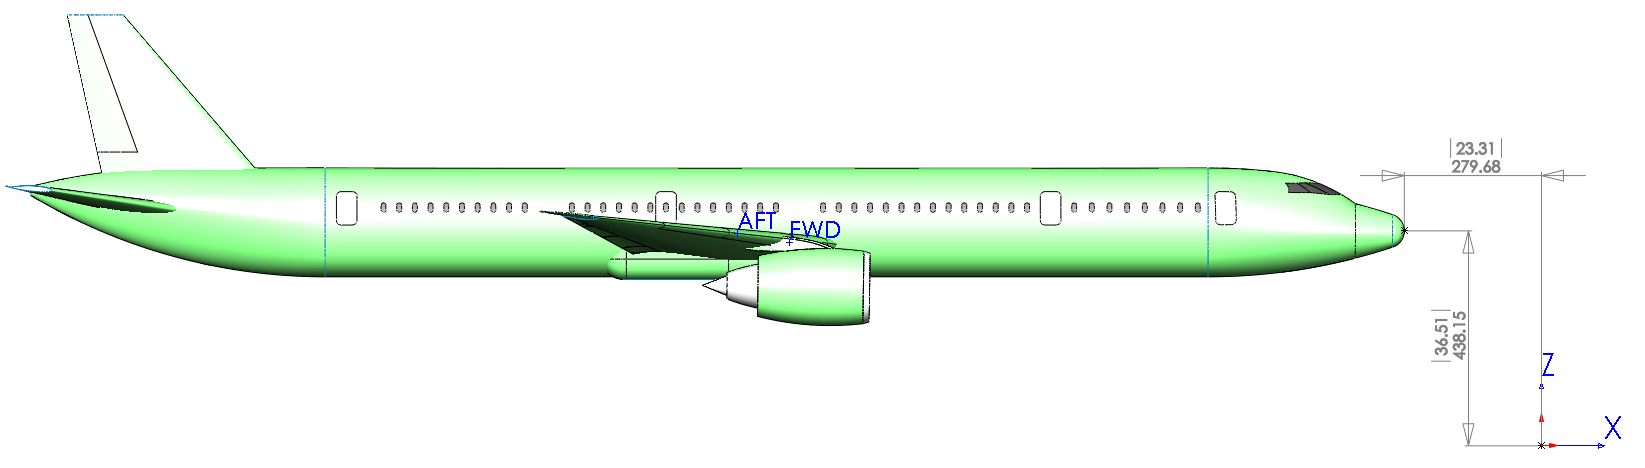
\includegraphics[width=\linewidth]{Photos/massprops/CG Side View.PNG}
    \caption{Definition of the Aircraft Coordinate System}
    \label{fig:master_coord_def}
\end{figure}
\FloatBarrier

\clearpage
The location of the CG limit defined by the MTOW condition and the empty weight condition is also depicted in Fig. \ref{fig:master_coord_def}. In Table \ref{tab:cg_final}, the CG location relative to the aircraft frame, as well as a function of \%MAC is tabulated for the MTOW, empty weight, and max zero fuel weight (MZFW) conditions.

\begin{table}[!h]
\centering
\caption{Location of CG Limits at Different Load Cases}
\begin{tabular}{|l||l|l|l|}
\hline
 & \textbf{MTOW} & \textbf{Empty Weight} & \textbf{MZFW} \\ \hline \hline
\textbf{X from Coordinate System (ft)} & -136.5 & -127.7 & -129.4 \\ \hline
\textbf{Z from Coordinate System (ft)} & 36.0 & 34.5 & 35.5 \\ \hline
\textbf{\% MAC} & 36.84\% & 2.21\% & 8.88\% \\ 
\bottomrule
\end{tabular}
\label{tab:cg_final}
\end{table}

\subsection{Effect of Material Composition of Center of Gravity and Weight of Aircraft}
The effect of different structure material composition was studied to see the how the weight and location of the aircraft changes as different structures of the aircraft change. The three different cases defined in Section \ref{section: strcuture material}: metallic, composite, and hybrid, were studied. The total weight of the aircraft at different cases is tabulated in Table \ref{tab:mass_study}. 

\begin{table}[!h]
\centering
\caption{Trade Study of Effect of Material Composition on Weight}
\label{tab:mass_study}
\begin{tabular}{|l||l|l|l|l|l|}
\hline
                              & \textbf{Metallic (lb)} & \textbf{Composite (lb)} & \textbf{Hybrid (lb)} & \textbf{$\Delta$ Metallic} & \textbf{$\Delta$ Composite} \\ \hline \hline
\textbf{Empty Weight}         & 227,500                & 207,900                 & 216,200              & 5.23\%                  & -3.84\%                  \\ \hline
\textbf{MTOW}                 & 468,700                & 449,100                 & 457,400              & 2.47\%                  & -1.81\%                  \\ \hline
\textbf{Max Zero Fuel Weight} & 321,840                & 302,200                 & 310,540              & 3.64\%                  & -2.69\%                  \\ \hline
\textbf{Max Landing Weight}   & 410,200                & 393,000                 & 400,300              & 2.47\%                  & -1.82\%                  \\ \hline
\textbf{Landing Weight}       & 321,840                & 302,200                 & 310,540              & 3.64\%                  & -2.69\%                  \\ \bottomrule
\end{tabular}
\end{table}

It can be noted that the metallic structure is heavier than the hybrid structure, and the composite structure is lighter. These calculations are using the assumptions made earlier in Table \ref{tab:mass_props}. The location of the CG for each material build-up as a function of \%MAC for the MTOW and empty weight conditions is tabulated in Table \ref{tab:mass_study2}.

\begin{table}[!h]
\centering
\caption{Trade Study of Effect of Material Composition on Location of CG}
\label{tab:mass_study2}
\begin{tabular}{|c|l||l|l|l|l|l|}
\hline
\multicolumn{2}{|l||}{}                                   & \textbf{Metallic   (lb)} & \textbf{Composite (lb)} & \textbf{Hybrid (lb)} & \textbf{$\Delta$ Metallic} & \textbf{$\Delta$ Composite} \\ \hline \hline
\multirow{2}{*}{\textbf{\% MAC}} & \textbf{MTOW}         & 39.56\%                  & 37.44\%                 & 36.84\%              & -2.72\%                 & -0.60\%                  \\ \cline{2-7} 
                                 & \textbf{Empty Weight} & 9.54\%                   & 2.11\%                  & 2.21\%               & -7.33\%                 & 0.11\%                   \\ \bottomrule
\end{tabular}
\end{table}

It can be noted that the metallic structure has a more aft empty weight and MTOW CG limit than both the composite and hybrid construction cases, and the composite CG limits are very similar to those of hybrid design.

\subsection{Center of Gravity Envelope}
When determining the stability of the aircraft, an envelope which contains the location of the center of gravity in relation to the MAC during loading of the payload, baggage, and fuel must be created. In Fig. \ref{fig:cg_envelope}, the envelope of the center of gravity of the SAM Mk. I is depicted.

\begin{figure}[!h]
    \centering
    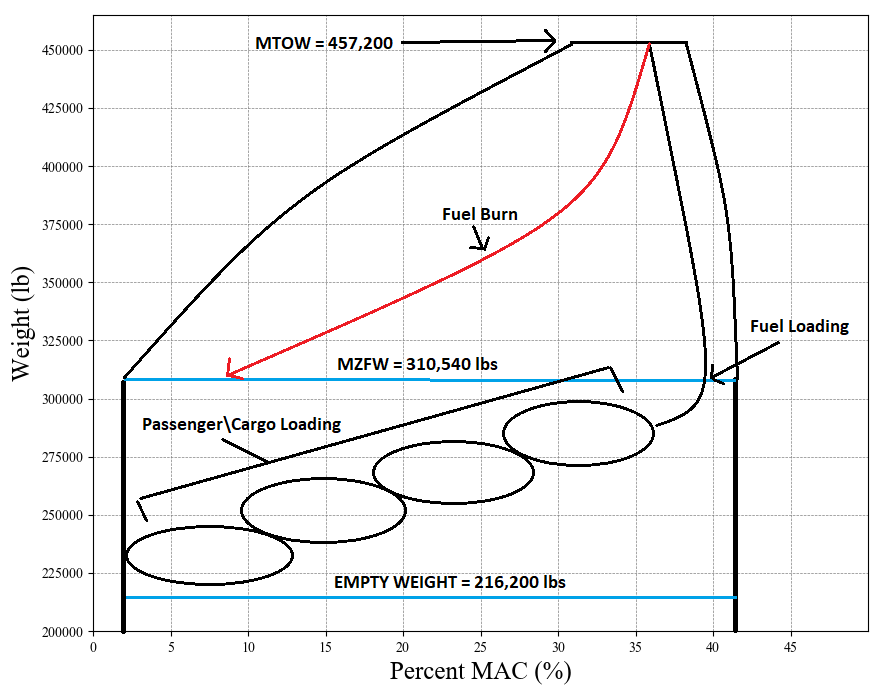
\includegraphics[width=\linewidth]{Photos/massprops/CG Envelope.png}
    \caption{Center of Gravity Envelope of the SAM Mk. I}
    \label{fig:cg_envelope}
\end{figure}

It can be noticed that the envelope spans from 2\% to 42\% MAC, which is in the range of the stability of the aircraft given the location of the landing gear, seen in Section \ref{section: Landing Gear}. As the fuel burns, the CG moves toward the MZFW location of 8.88 \%MAC.





% \textcolor{red}{
% \begin{itemize}
% \item Discuss any analysis supporting the sizing analysis.
% \begin{itemize}
% \item Mass property methods chosen for different parts of the aircraft.
% \item Estimate CG location.
% \end{itemize}
% \item Discuss future work.
% \item AIAA: Aircraft weight statement, aircraft center-of-gravity envelope reflecting payloads and fuel allocation. Establish a forward and aft center of gravity (CG) limits for safe flight. (may come later...con't on AIAA doc \href{https://www.aiaa.org/docs/default-source/uploadedfiles/education-and-careers/university-students/design-competitions/undergraduate-team-aircraft-design-competition/undergraduate-aircraft-high-capacity-short-range-transport-aircraft.pdf?sfvrsn=b6081273_0}{here}: )
% \end{itemize}}